\documentclass[border=1pt]{standalone}
\usepackage[dvipsnames]{xcolor}
\usepackage{tikz}                       % Graphen und kommutative Diagramme
\usetikzlibrary{patterns}               % Um schraffierte Formen in der tikzpicture-Umgebung zu zeichnen.

\begin{document}

\newcommand{\ul}{\underline}
\newcommand{\radmult}
{
    \ensuremath{
	\tikz[baseline={([yshift=-1pt]current bounding box.center)}, x=5pt, y=2.5pt, every node/.style={shape=circle, fill=black, inner sep=.9pt}]{
	    \draw[line width=0.9pt] (5, 0) -- (3, 0);
	    \draw[line width=0.9pt] (2, 0) -- (0, 0);
	    \filldraw (3, 0) circle (1pt);
	    \filldraw (2, 0) circle (1pt);
	}
    }
    
    
    
}

\newcommand{\equals}
{
    \ensuremath{
	\tikz[baseline={([yshift=2pt]current bounding box.center)}, x=5pt, y=2.5pt]{
	    \node (0, 0) {$=$};
	}
    }
}

\centering
\begin{minipage}{.55\textwidth}
\centering
\resizebox{!}{6.5cm}{
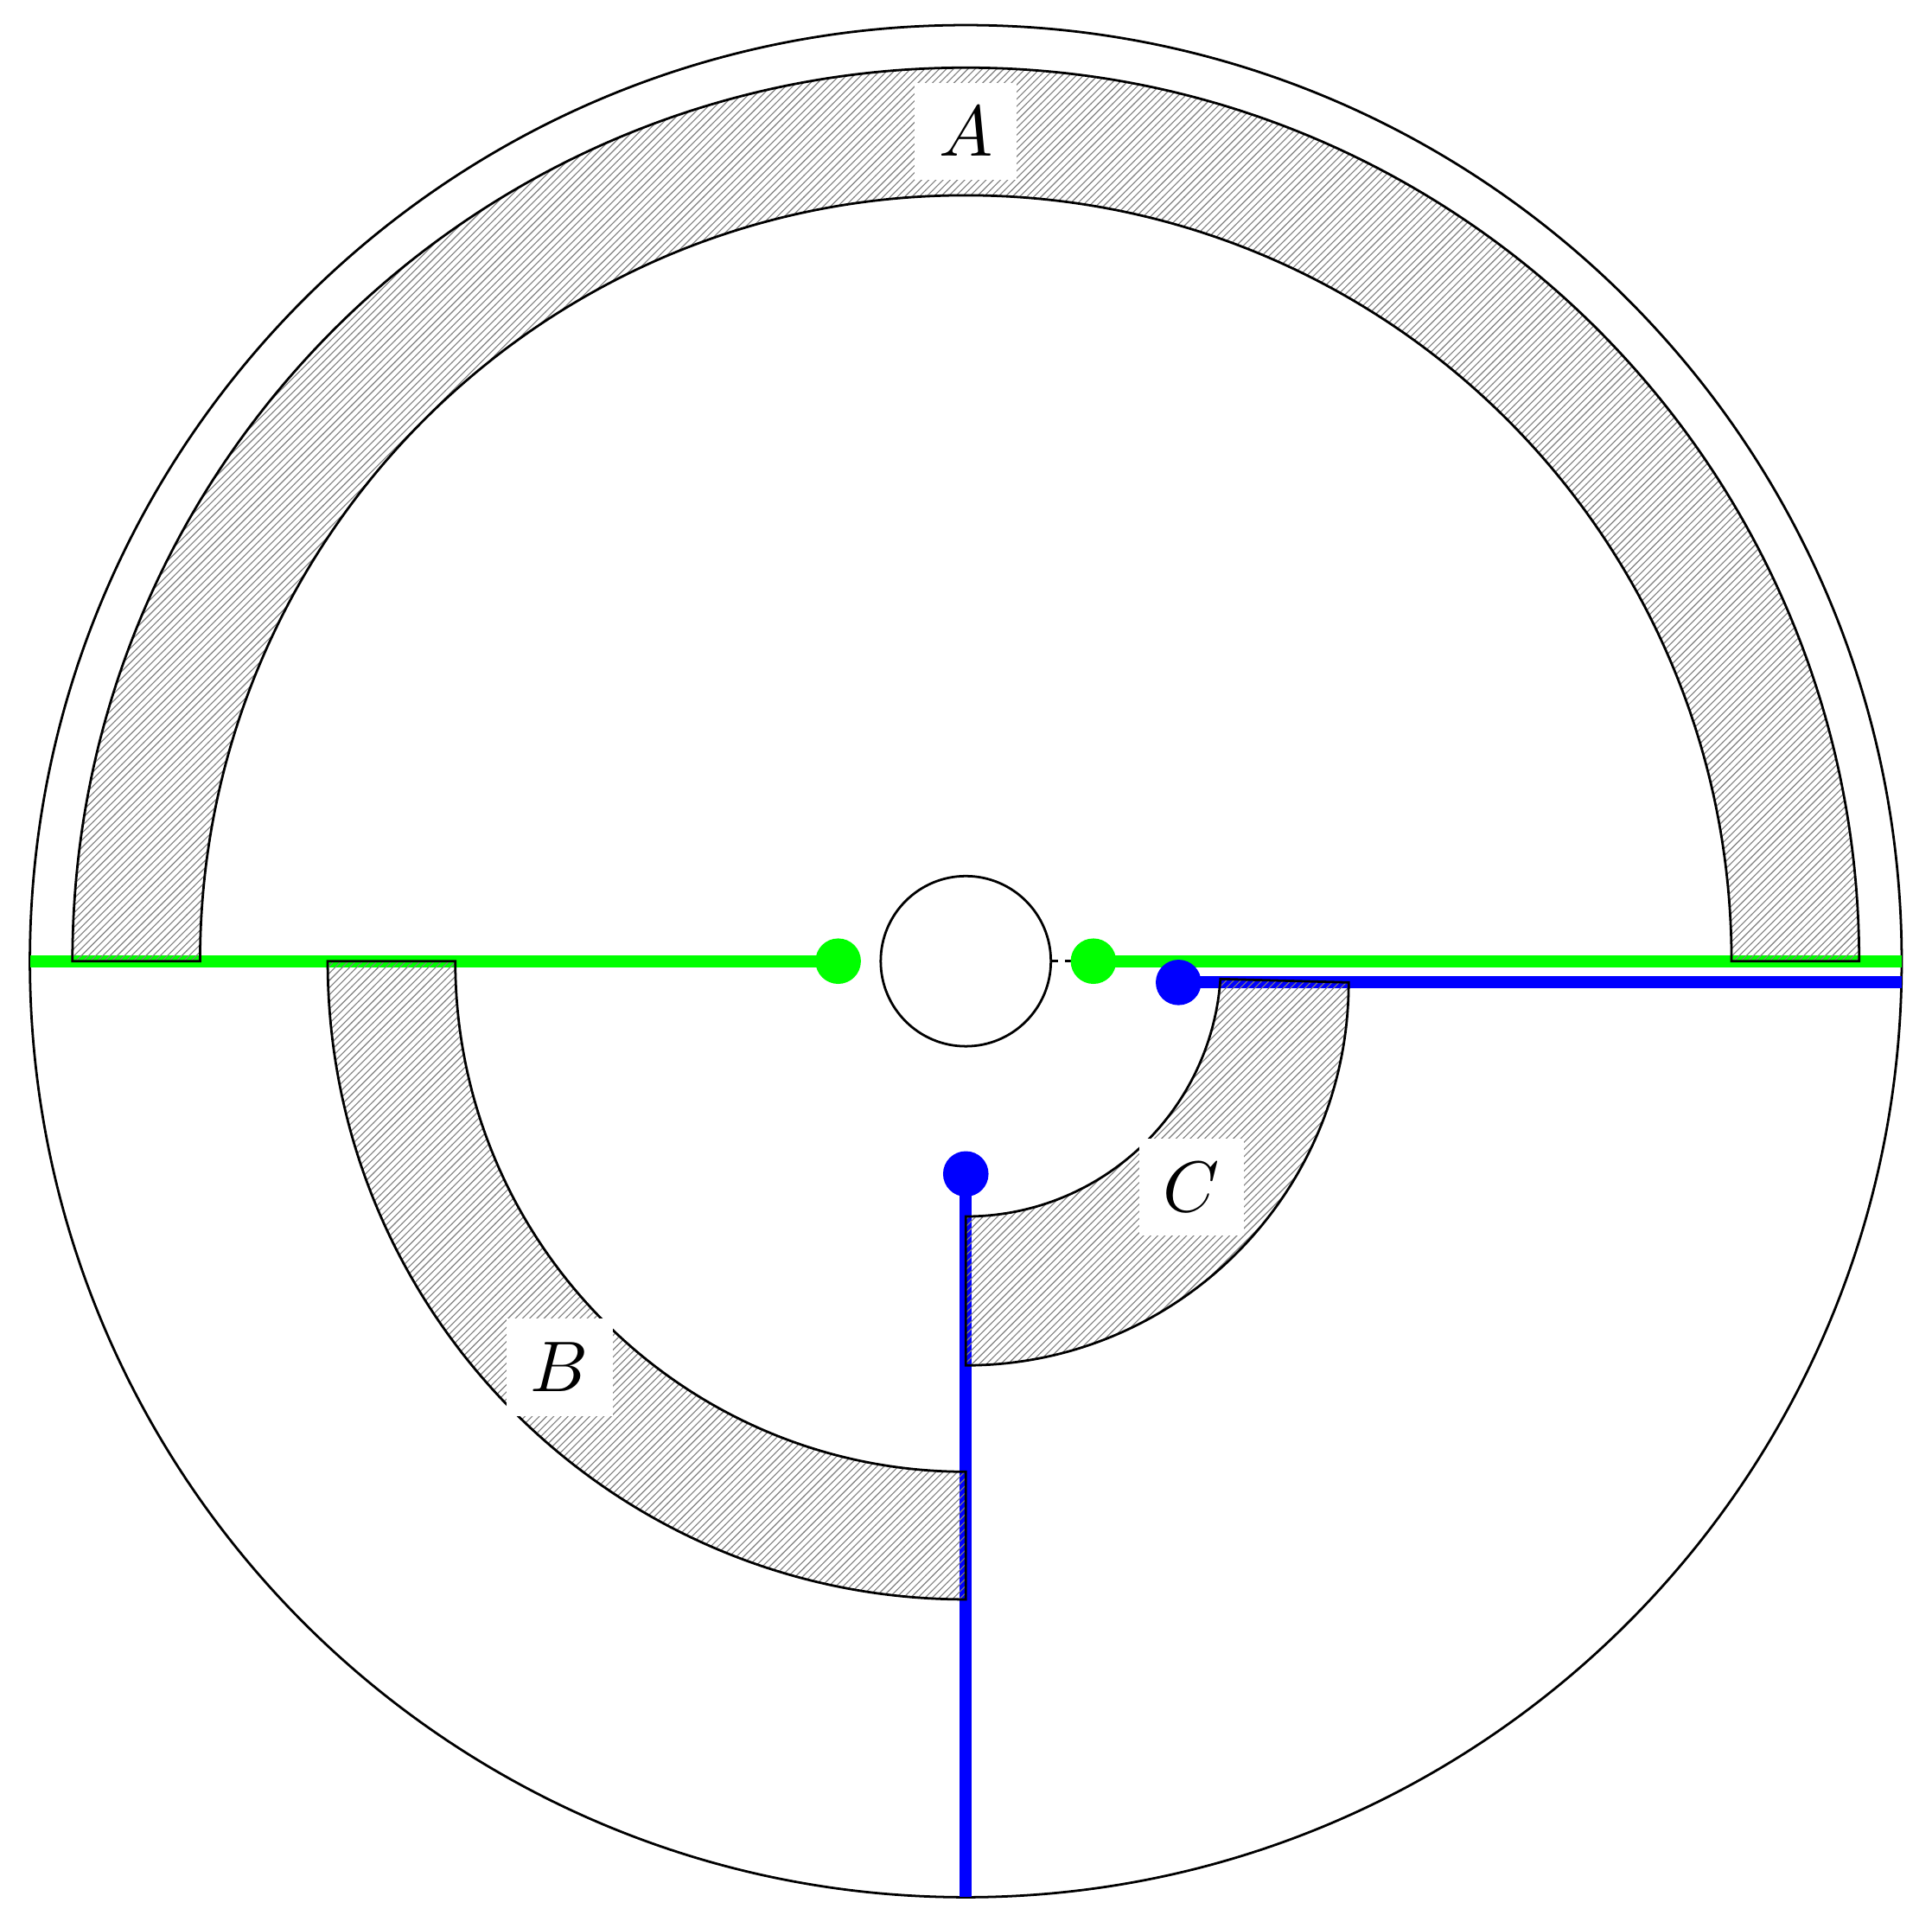
\begin{tikzpicture}[x=1.25cm, y=1.25cm, line width=1pt]

% draw inner and outer circle
\draw[color=black] (0, 0) circle (1);
\draw[color=black] (0, 0) circle (11);

% draw 0 line
\draw[dashed] (0 : 1) -- ( 0: 11);

% draw slits
\draw[color = green, line width=5pt] (0 : 1.5) -- (0 : 11);
\draw[color = green, line width=5pt] (180 : 1.5) -- (180 : 11);
\filldraw[color = green, fill = green] (0 : 1.5) circle (9pt);
\filldraw[color = green, fill = green] (180 : 1.5) circle (9pt);

\draw[color=blue, line width=5pt] (270 : 2.5) -- (270: 11);
\draw[color=blue, line width=5pt] (2.5, -0.25) -- (11, -0.25);
\filldraw[color = blue, fill = blue] (270: 2.5) circle (9pt);
\filldraw[color = blue, fill = blue] (2.5, -0.25) circle (9pt);

% draw shaded concentrical stripes
\filldraw[pattern=north east lines, pattern color=black!50] (180 : 9) arc [radius = 9, start angle = 180, delta angle = -180]
                                                     -- (0 : 10.5) arc [radius = 10.5, start angle = 0, delta angle = 180]
                                                     -- cycle;
                                                     
\filldraw[pattern=north east lines, pattern color=black!50] (270 : 6) arc [radius = 6, start angle = 270, delta angle = -90]
                                                     -- (180 : 7.5) arc [radius = 7.5, start angle = 180, delta angle = 90]
                                                     -- cycle;

\filldraw[pattern=north east lines, pattern color=black!50] (4.5, -0.25) arc [radius = 4.5, start angle = 0, delta angle = -90]
                                                     -- (270 : 3) arc [radius = 3, start angle = 270, delta angle = 86]
                                                     -- cycle;
                                                     
% draw labels
\node[scale = 3, fill = white] at (90 : 9.75) {$A$};
\node[scale = 3, fill = white] at (225 : 6.75) {$B$};
\node[scale = 3, fill = white] at (315 : 3.75) {$C$};

\end{tikzpicture}
}
\end{minipage}

\centering
\begin{minipage}{.55\textwidth}
\centering
\resizebox{!}{6.5cm}{
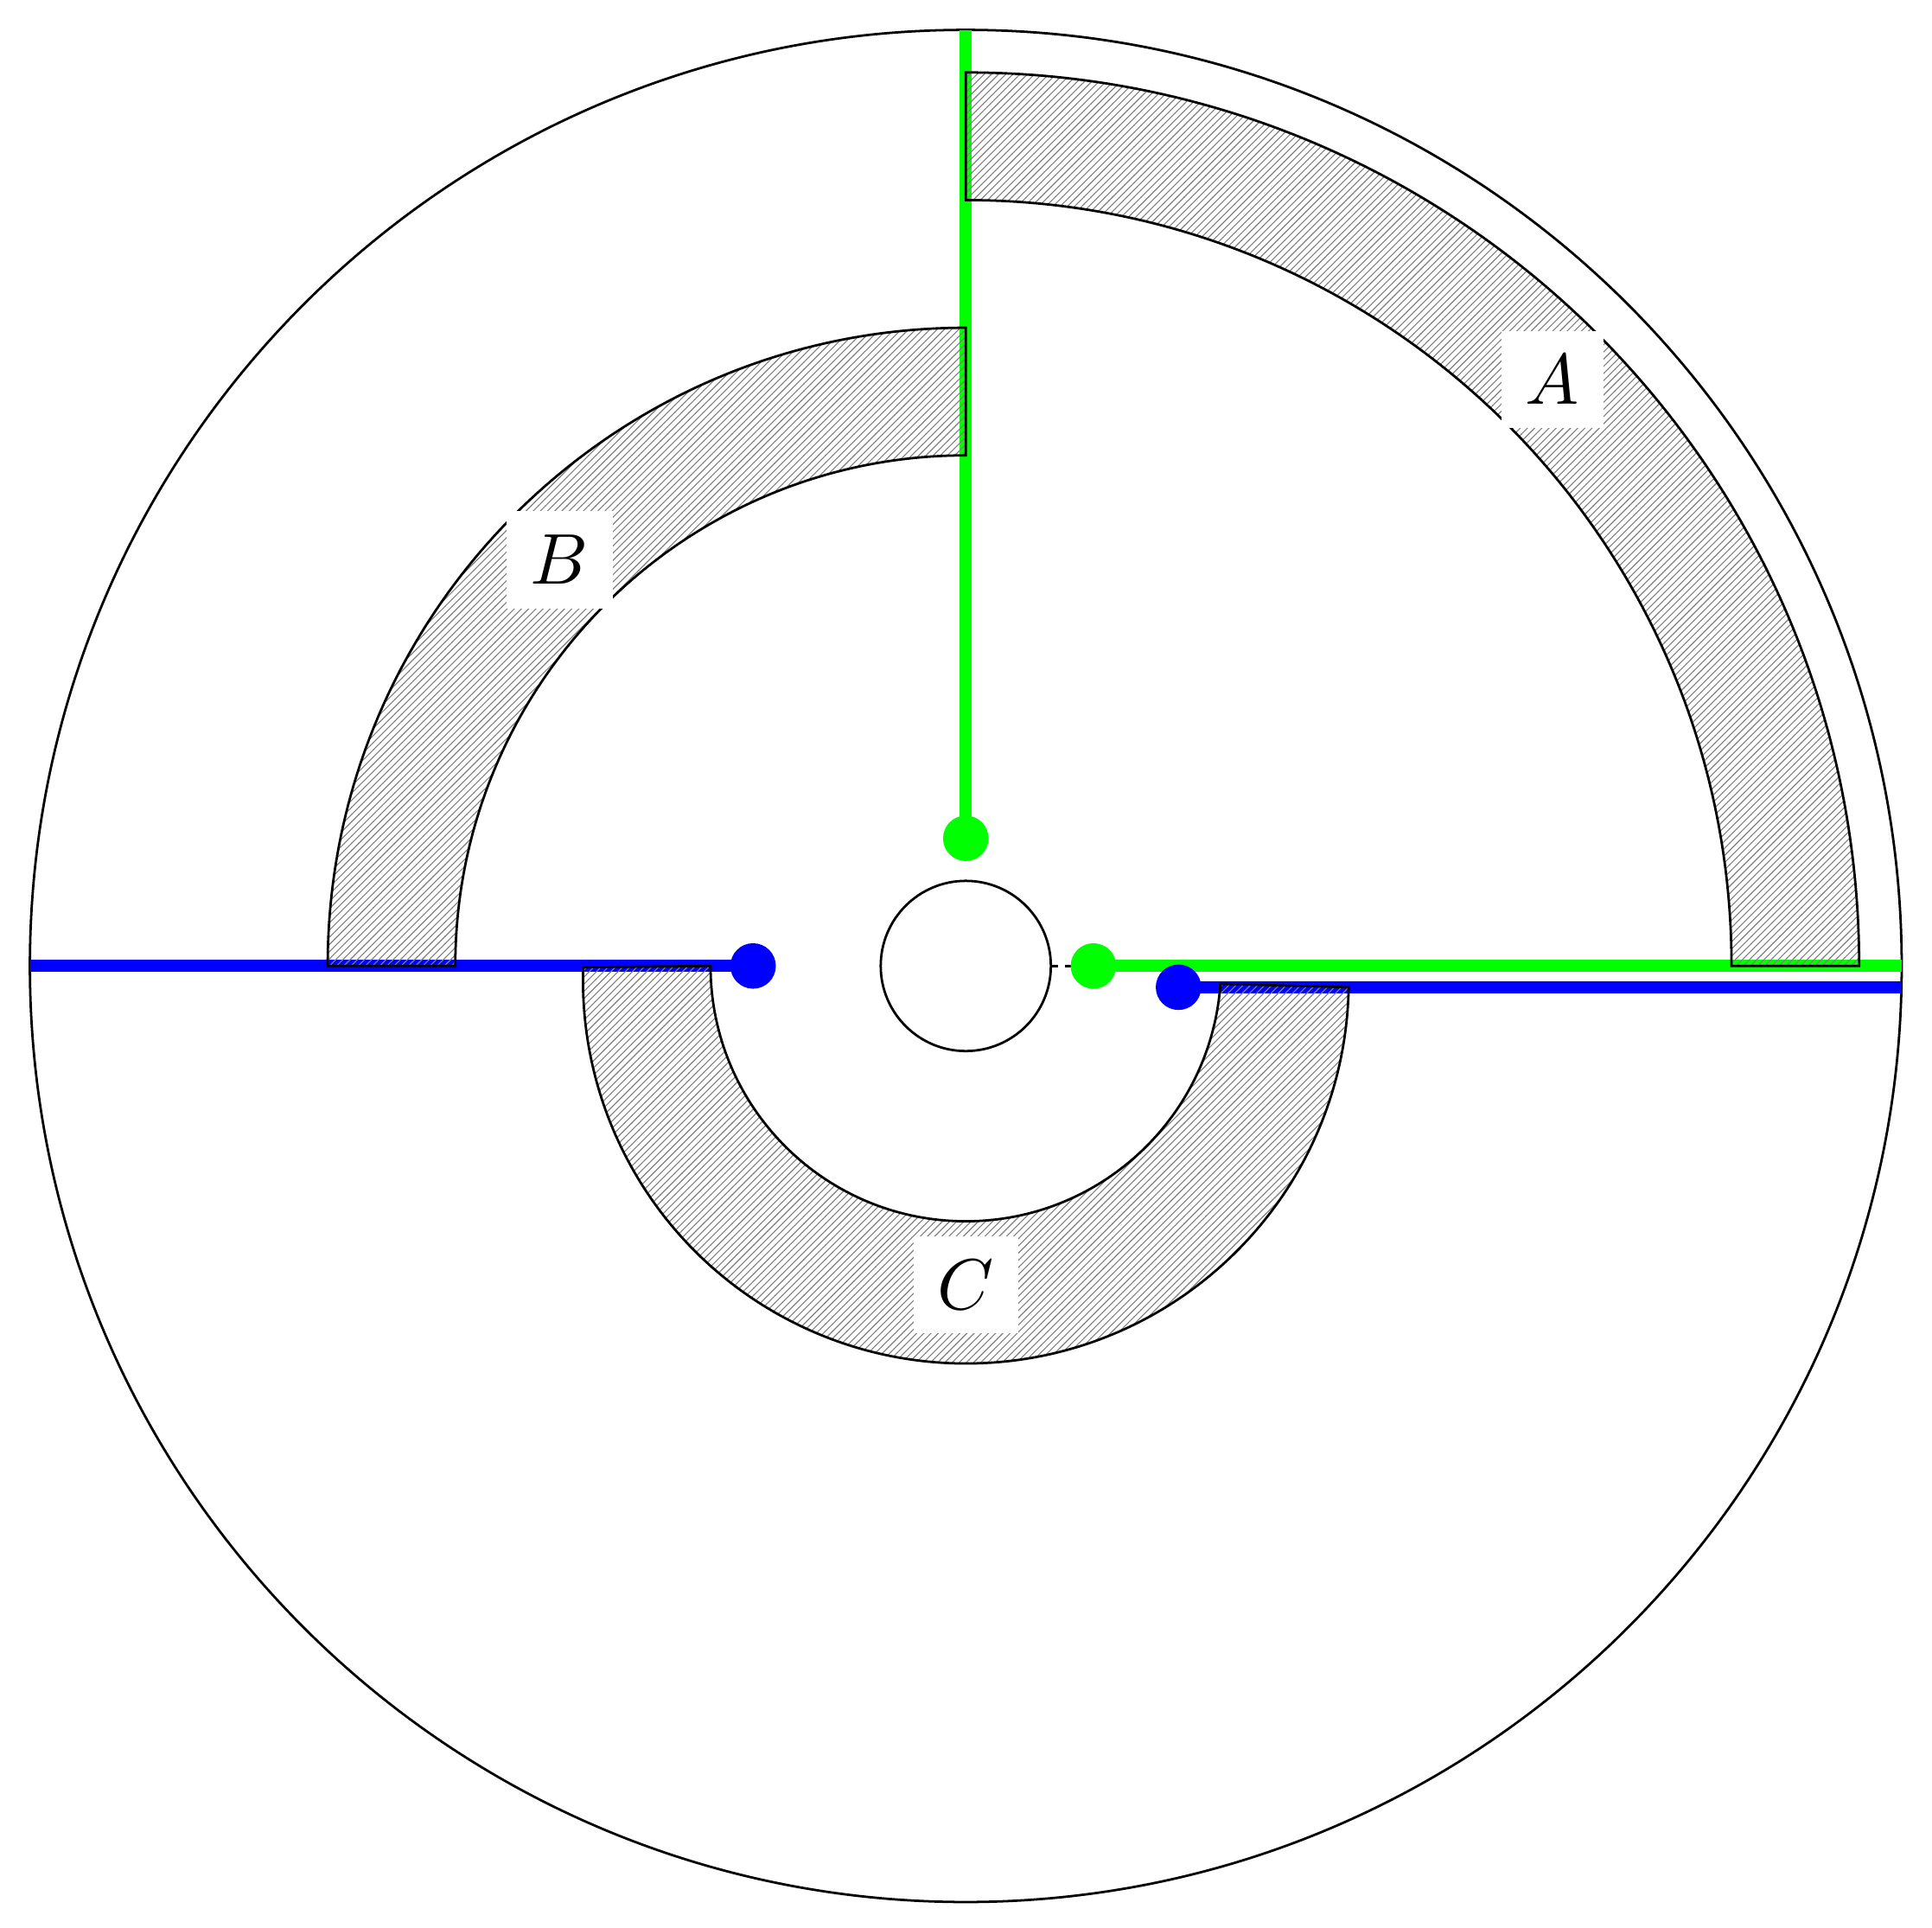
\begin{tikzpicture}[x=1.25cm, y=1.25cm, line width=1pt]

% draw inner and outer circle
\draw[color=black] (0, 0) circle (1);
\draw[color=black] (0, 0) circle (11);

% draw 0 line
\draw[dashed] (0 : 1) -- ( 0: 11);

% draw slits
\draw[color=green, line width=5pt] (0 : 1.5) -- (0 : 11);
\draw[color=green, line width=5pt] (90 : 1.5) -- (90 : 11);
\filldraw[color = green, fill = green] (0 : 1.5) circle (9pt);
\filldraw[color = green, fill = green] (90 : 1.5) circle (9pt);

\draw[color=blue, line width=5pt] (180 : 2.5) -- (180: 11);
\draw[color=blue, line width=5pt] (2.5, -0.25) -- (11, -0.25);
\filldraw[color = blue, fill = blue] (180: 2.5) circle (9pt);
\filldraw[color = blue, fill = blue] (2.5, -0.25) circle (9pt);

% draw shaded concentrical stripes
\filldraw[pattern=north east lines, pattern color=black!50] (90 : 9) arc [radius = 9, start angle = 90, delta angle = -90]
                                                     -- (0 : 10.5) arc [radius = 10.5, start angle = 0, delta angle = 90]
                                                     -- cycle;
                                                     
\filldraw[pattern=north east lines, pattern color=black!50] (180 : 6) arc [radius = 6, start angle = 180, delta angle = -90]
                                                     -- (90 : 7.5) arc [radius = 7.5, start angle = 90, delta angle = 90]
                                                     -- cycle;

\filldraw[pattern=north east lines, pattern color=black!50] (4.5, -0.25) arc [radius = 4.5, start angle = 359, delta angle = -181]
                                                     -- (180 : 3) arc [radius = 3, start angle = 180, delta angle = 176]
                                                     -- cycle;
                                                     
% draw labels
\node[scale = 3, fill = white] at (45 : 9.75) {$A$};
\node[scale = 3, fill = white] at (135 : 6.75) {$B$};
\node[scale = 3, fill = white] at (270 : 3.75) {$C$};

\end{tikzpicture}
}
\end{minipage}

\end{document}